% IEEEtran 1.8b, original class in vendor/IEEEtran, conference defaults retained.
% Compile with tools/build.py; direct final compilation is deliberately blocked.
\documentclass[conference]{vendor/IEEEtran/IEEEtran}
\IEEEoverridecommandlockouts
\usepackage[T1]{fontenc}
\usepackage[brazil]{babel}
\usepackage{graphicx}
\usepackage{booktabs}
\usepackage{amsmath}
\usepackage{cite}
\usepackage[hidelinks]{hyperref}
\usepackage{url}
\graphicspath{{figures/}}

\ifdefined\AiiDraft
  \providecommand{\PublicRepositoryURL}{ENDERECO-PUBLICO-PENDENTE}
\else
  \ifdefined\AiiFinalConfigured\else
    \PackageError{A2}{Versao final bloqueada: use tools/build.py --final}{URL publica, resultados novos e verificacoes sao obrigatorios.}
  \fi
\fi
\newcommand{\pendente}[1]{\textbf{[PENDENTE: #1]}}
\newcommand{\fisio}{\textsc{Fisio8}}
\newcommand{\strict}{\textsc{Strict4}}
\hypersetup{pdftitle={Classificacao de registros clinicos com auditoria de vazamento},
  pdfauthor={Antonio Henrique Queiroz Villar Lopes; Joao Vitor Fernandes Ferreira; Mateus Nery Bailao; Pedro Augusto Ferreira Matos},
  pdflang={pt-BR}}

\title{Classificação de registros clínicos com auditoria de vazamento de informação\thanks{Repositório público e código reprodutível: \expandafter\url\expandafter{\PublicRepositoryURL}.}}
\author{\IEEEauthorblockN{Antônio Henrique Queiroz Villar Lopes, João Vitor Fernandes Ferreira\\
Mateus Nery Bailão, Pedro Augusto Ferreira Matos}
\IEEEauthorblockA{Instituto de Informática, Universidade Federal de Goiás (UFG)\\Mineração de Dados (2026/2), Goiânia, Brasil}}

\begin{document}
\maketitle
\ifdefined\AiiDraft
\begin{center}\textbf{VERSÃO DE TRABALHO: NÃO SUBMETER}\end{center}
\fi
\begin{abstract}
Investigamos a classificação binária do rótulo cardíaco registrado na base pediátrica UCMF, com atenção à possibilidade de vazamento de informação. Auditamos os 21 atributos e excluímos dos preditores motivos de encaminhamento com conteúdo diagnóstico, achados do exame cardiovascular e campos de proveniência incerta. Com 9.361 registros de desenvolvimento, comparamos uma referência majoritária, árvore de decisão, regressão logística e floresta aleatória em validação cruzada aninhada, estratificada e agrupada. Imputação, codificação e escalonamento foram ajustados em cada treino. A floresta alcançou acurácia balanceada de 62,87\% e sensibilidade de 59,29\% no cenário fisiológico. Com quatro atributos antropométricos e demográficos, a regressão logística obteve a maior acurácia balanceada, de 59,74\%. A mudança na ordenação das famílias indica dependência do conjunto de entradas. A cronologia da coleta e a origem do rótulo limitam a interpretação clínica.

\end{abstract}
\begin{IEEEkeywords}
classificação, dados clínicos, validação cruzada, vazamento de informação.
\end{IEEEkeywords}

\section{Introdução}
A base UCMF reúne registros de atendimento cardiológico pediátrico. O dicionário descreve a variável \textit{NORMAL X ANORMAL} em termos de presença ou ausência de patologia cardíaca \cite{tema,dict}. Consideramos \textit{Anormal} a classe positiva e investigamos em que medida características antropométricas, demográficas e fisiológicas discriminam esse rótulo. A fonte disponível deixa em aberto a ordem de registro dos campos, a identidade do responsável pela rotulagem e o padrão diagnóstico de referência. Essas lacunas afetam tanto a escolha dos preditores quanto o significado dos resultados.

Na avaliação anterior, o trabalho chegou à transformação dos dados. Nesta A2, revimos seleção, limpeza e transformação e completamos a mineração e a interpretação do processo KDD. O desenho compara famílias de modelos sob as mesmas partições e usa dois conjuntos de atributos para avaliar quanto a conclusão depende de medidas mais próximas da avaliação cardiovascular.

\section{Dados e análise exploratória}
\begin{figure*}[!t]
\centering
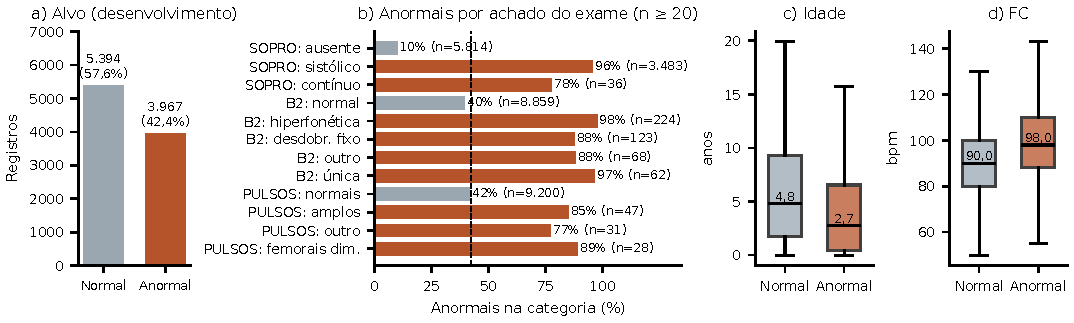
\includegraphics[width=\textwidth]{eda_alvo_achados.pdf}
\caption{Conjunto de desenvolvimento. (a) Distribuição do alvo. (b) Percentual de anormais em cada categoria de SOPRO, B2 e PULSOS com pelo menos 20 registros; a linha tracejada marca a proporção geral (\pctAnormal\%). (c, d) Idade e frequência cardíaca por classe; as caixas vão do primeiro ao terceiro quartil, o traço é a mediana e os pontos atípicos não são desenhados.}
\label{fig:eda}
\end{figure*}

\subsection{Origem e composição}
A fonte tem \recNSource{} registros e 21 atributos \cite{tema,dict}: identificação (ID, Atendimento, DN), antropometria (Peso, Altura, IMC), IDADE, SEXO, sinais vitais (pressões sistólica e diastólica, PAS e PAD, e frequência cardíaca, FC), a classificação de pressão arterial PPA \cite{ppa}, achados do exame físico (SOPRO, segunda bulha B2 e PULSOS), sintomas da história da doença atual (HDA1 e HDA2), Convênio, os motivos de encaminhamento (MOTIVO1 e MOTIVO2) e o alvo. Há \recNUnlabelled{} registros sem rótulo, que ficam fora da classificação supervisionada. Dos \recNLabelledAdois{} rotulados, \nDev{} formam o conjunto de desenvolvimento e \nTest{} formam o teste histórico, separado em uma fase anterior do projeto; \nRetirado{} registro idêntico a outro do teste foi retirado do desenvolvimento. O desenvolvimento tem \nNormal{} registros \textit{Normal} e \nAnormal{} \textit{Anormal} (\pctAnormal\%), um desequilíbrio moderado (Fig.~\ref{fig:eda}a).

\subsection{Descobertas da análise exploratória}
Os achados do exame físico separam as classes com nitidez (Fig.~\ref{fig:eda}b). Entre os \sopSisN{} registros com sopro sistólico, \sopSisPct\% são anormais; entre os \sopAusN{} sem sopro, \sopAusPct\%. B2 normal tem \btwoNormPct\% de anormais e B2 hiperfonética, \btwoHiperPct\%. Pulsos alterados também se concentram na classe anormal, mas são raros.

As crianças com rótulo anormal são mais novas (Fig.~\ref{fig:eda}c): a mediana de idade é \idadeMedAnormal{} anos contra \idadeMedNormal{}, e \menosUmAnoAnormal\% dos anormais têm menos de um ano, contra \menosUmAnoNormal\% dos normais. A FC mediana é \fcMedAnormal{} bpm nos anormais e \fcMedNormal{} bpm nos normais, com intervalos interquartis sobrepostos (\fcQumAnormal--\fcQtresAnormal{} e \fcQumNormal--\fcQtresNormal{} bpm). Como a FC de repouso cai com a idade, parte dessa diferença acompanha a idade.

A falta de dados é desigual: PAS falta em \missPAS\% dos registros, PPA em \missPPA\%, HDA1 em \missHDAum\% e HDA2 em \missHDAdois\%, enquanto SOPRO, B2 e PULSOS faltam em menos de 1\%.

\subsection{Vazamento de informação}
Consideramos vazamento todo atributo indisponível no momento da previsão ou que já contenha a conclusão diagnóstica. A Tabela~\ref{tab:policy} resume a decisão para os 21 atributos. MOTIVO1 e MOTIVO2 trazem textos como ``cardiopatia já estabelecida'' e ``cardiopatia congênita''; a A1 já havia apontado esse risco, e cada um sozinho atinge acurácia balanceada (BA) de \probeMotivoUm\% e \probeMotivoDois\% em um teste exploratório com uma árvore rasa. Convênio descreve a origem do paciente e o caminho de encaminhamento, não a criança: os \susN{} registros do SUS no desenvolvimento têm \susPct\% de anormais, o que reflete quem encaminha, e não o que se observa no atendimento. HDA2 tem \missHDAdois\% de ausentes e sai pela regra da A1 de excluir atributos com mais de 50\% de ausência.

Os achados de exame (SOPRO, B2, PULSOS), os sintomas relatados (HDA1) e a PPA, calculada a partir de PAS, PAD, idade, sexo e altura \cite{ppa}, são coletados durante o atendimento, antes do laudo. São exatamente a informação que o cardiologista usa para decidir a investigação \cite{guideline}. SOPRO sozinho atinge BA de \probeSopro\% no mesmo teste exploratório; isso mede poder preditivo de um dado disponível, não vazamento. O cenário principal, \clinico{}, mantém esses atributos. Os cenários \fisio{} e \strict{} servem de análise de sensibilidade: retiram os achados de exame e, no segundo caso, também os sinais vitais.

\begin{table}[!t]
\centering
\caption{Decisão sobre os 21 atributos originais}
\label{tab:policy}
\footnotesize
\begin{tabular}{@{}p{0.36\columnwidth}p{0.59\columnwidth}@{}}
\toprule
Atributos & Decisão \\
\midrule
\textit{NORMAL X ANORMAL} & Alvo. \\
ID & Fora: identificador. \\
Atendimento, DN & Fora como datas; usadas para conferir IDADE. \\
Convênio & Fora: origem do paciente, não achado clínico. \\
MOTIVO1, MOTIVO2 & Fora: conteúdo diagnóstico explícito. \\
HDA2 & Fora: mais de 50\% de ausentes. \\
SOPRO, B2, PULSOS, HDA1, PPA & Em \clinico{}: coletados antes do laudo. \\
IMC, PAS, PAD, FC & Em \clinico{} e \fisio{}. \\
Peso, Altura, IDADE, SEXO & Nos três cenários. \\
\bottomrule
\end{tabular}
\end{table}

\section{Metodologia}
\subsection{Limpeza e transformação}
A fonte foi preservada. Padronizamos grafias, separadores decimais e códigos de ausência, convertendo as medidas às unidades do dicionário. As regras por registro usam coerência entre campos e limites amplos de plausibilidade. Medidas suspeitas são mascaradas com registro da regra. Conservar a linha permite usar suas demais informações. A correção de altura em centímetros depende da coerência com a escala do campo. Para IMC, usamos a relação peso dividido pela altura em metros ao quadrado quando ambos os insumos são válidos, com preservação controlada do valor histórico quando essa reconstrução é inviável. Para IDADE, a diferença entre nascimento e atendimento é usada quando a interpretação das datas é coerente. O valor informado tem papel de referência nas ambiguidades de formato e século. As regras e exceções por variável foram documentadas na auditoria.

Em cada treino, comparamos a mediana global com medianas em faixas fixas de idade para Peso, Altura, IMC e FC quando presentes. A faixa requer pelo menos 30 valores observados no treino. Caso contrário ou com idade indisponível, vale a mediana global. O indicador de imputação numérica conserva informação sobre indisponibilidade e o ensaio de máscaras investiga seu poder preditivo. SEXO usa codificação \textit{one-hot} com vocabulário do treino. Para a logística comparamos padronização das medidas originais com a padronização após aplicar \(\log(1+\text{Peso})\) ao Peso. As árvores usam as unidades originais. Indicadores binários permanecem em sua escala. Nenhum parâmetro de transformação é estimado nas linhas de validação.

\subsection{Mineração e avaliação}
O cenário \fisio{} usa Peso, Altura, IMC, IDADE, pressões sistólica e diastólica, FC e SEXO. \strict{} usa Peso, Altura, IDADE e SEXO. A segunda análise reduz a dependência de medidas cardiovasculares cuja relação com a rotulagem é incerta e elimina a redundância de IMC com os insumos antropométricos. Os dois cenários compartilham os mesmos registros e cortes externos.

Usamos a classe majoritária como referência, uma árvore rasa como comparação interpretável, regressão logística regularizada e floresta aleatória \cite{breiman2001,pedregosa2011}. A grade por cenário inclui 105 configurações. São 48 de árvore (critério, profundidade, tamanho mínimo de folha, pesos e imputação), 32 de logística (regularização, representação, pesos e imputação), 24 de floresta (profundidade, folha mínima, pesos e imputação, com 150 árvores) e uma referência majoritária. Os pesos balanceados aumentam a contribuição da classe menos frequente no treino. A busca compara seu efeito com pesos uniformes. O limiar de 0,5 é fixado para a comparação.

A validação cruzada aninhada separa ajuste e estimativa de desempenho \cite{varma2006}. Em cada um dos cinco folds externos, três folds internos escolhem uma configuração por família pela média da acurácia balanceada (BA). Em empate numérico, prevalece a ordem fixa da grade. O procedimento reajusta o vencedor no treino externo e gera uma previsão para cada linha de sua validação. A estratificação procura preservar as proporções de classe e o agrupamento evita separar componentes candidatos entre treino e validação. Usamos \texttt{random\_state=42} nos estimadores estocásticos, semente 743 nos cortes externos e \(811+k\) no corte interno do fold \(k\), com \(k=0,\ldots,4\).

A BA é a média da sensibilidade (fração de \textit{Anormal} recuperada) e da especificidade (fração de \textit{Normal} reconhecida). Ela dá o mesmo peso às classes. Relatamos também precisão da classe positiva, \(F_1\), precisão média (AP) e matriz de confusão. As métricas principais reúnem as previsões externas de todos os folds. O desvio-padrão entre folds descreve a variação observada. Como os treinos se sobrepõem, esse desvio não foi usado como erro-padrão de observações independentes.

\section{Resultados e discussão}
\begin{table}[!t]
\centering
\caption{Métricas das previsões externas da validação aninhada (\%)}
\label{tab:results}
\footnotesize
\setlength{\tabcolsep}{2.6pt}
\begin{tabular}{@{}llrrrrrrr@{}}
\toprule
Cenário & Família & BA & Sens. & Esp. & Prec. & \(F_1\) & AUC & AP \\
\midrule
\multirow{4}{*}{\textsc{Clinico}} & Maioria & 50,00 & 0,00 & 100,00 & 0,00 & 0,00 & 50,00 & 42,38 \\
 & Árvore & \textbf{91,94} & 87,50 & 96,38 & 94,68 & 90,95 & 92,29 & 91,38 \\
 & Logística & 91,90 & 87,40 & 96,40 & 94,70 & 90,90 & 94,02 & 93,70 \\
 & Floresta & 91,91 & 87,37 & 96,46 & 94,78 & 90,92 & 94,74 & 94,43 \\
\midrule
\multirow{4}{*}{\textsc{Fisio8}} & Maioria & 50,00 & 0,00 & 100,00 & 0,00 & 0,00 & 50,00 & 42,38 \\
 & Árvore & 60,91 & 54,32 & 67,50 & 55,14 & 54,73 & 63,68 & 56,00 \\
 & Logística & 61,64 & 55,51 & 67,78 & 55,89 & 55,70 & 65,64 & 56,67 \\
 & Floresta & \textbf{62,91} & 58,91 & 66,91 & 56,70 & 57,78 & 67,20 & 59,55 \\
\midrule
\multirow{4}{*}{\textsc{Strict4}} & Maioria & 50,00 & 0,00 & 100,00 & 0,00 & 0,00 & 50,00 & 42,38 \\
 & Árvore & 59,32 & 35,82 & 82,81 & 60,52 & 45,00 & 61,53 & 54,37 \\
 & Logística & \textbf{59,74} & 52,03 & 67,45 & 54,03 & 53,01 & 63,66 & 55,78 \\
 & Floresta & 59,67 & 49,61 & 69,73 & 54,65 & 52,01 & 64,35 & 57,46 \\
\bottomrule

\end{tabular}
\par\smallskip
\raggedright\scriptsize Sens.\ = sensibilidade; Esp.\ = especificidade; AUC = área sob a curva ROC. Maioria é o baseline simples. Em negrito, a maior BA de cada cenário. Precisão e \(F_1\) da maioria valem zero porque ela não prevê positivos.
\end{table}

\subsection{Comparação entre cenários e famílias}
A Tabela~\ref{tab:results} reúne as previsões externas dos \nDev{} registros de desenvolvimento. Em \clinico{}, árvore, logística e floresta ficam a \clinBAspread{} ponto percentual uma da outra em BA, um empate prático. Pelo critério fixado antes da execução, a árvore tem a maior BA (\vClinArvBA\%), com sensibilidade de \vClinArvSens\% e especificidade de \vClinArvEsp\%. A floresta ordena melhor as probabilidades (ROC-AUC de \vClinFloAUC\% contra \vClinArvAUC\% da árvore), o que importa se o limiar for ajustado. O modelo final da árvore usa \finalClinParams{} e \finalClinImput{}; com profundidade dois, ele equivale a uma regra sobre poucos atributos.

Retirar os achados de exame derruba o desempenho: a melhor BA cai \ganhoClinFisio{} pontos, para \vFisioFloBA\% (\bestFisio{} em \fisio{}). Retirar também os sinais vitais tira mais \ganhoFisioStrict{} pontos, para \vStrictLogBA\% (\bestStrict{} em \strict{}). Nos dois cenários de sensibilidade, os modelos superam o baseline, mas discriminam pouco.

\begin{table}[!t]
\centering
\caption{Matrizes de confusão das previsões externas}
\label{tab:confusion}
\footnotesize
\begin{tabular}{@{}lrrrr@{}}
\toprule
& \multicolumn{2}{c}{\clinico{} (árvore)} & \multicolumn{2}{c}{\fisio{} (floresta)} \\
\cmidrule(lr){2-3}\cmidrule(l){4-5}
Rótulo & Normal & Anormal & Normal & Anormal \\
\midrule
Normal & \vClinArvTN & \vClinArvFP & \vFisioFloTN & \vFisioFloFP \\
Anormal & \vClinArvFN & \vClinArvTP & \vFisioFloFN & \vFisioFloTP \\
\bottomrule
\end{tabular}
\par\smallskip
\raggedright\scriptsize Linhas: rótulo registrado. Colunas: classe prevista.
\end{table}

\begin{figure*}[!t]
\centering
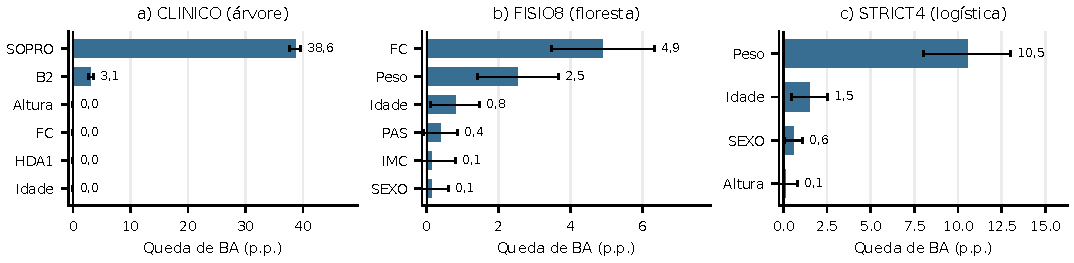
\includegraphics[width=\textwidth]{importancia.pdf}
\caption{Importância por permutação no modelo de maior BA de cada cenário: queda média de BA ao embaralhar o atributo no \textit{fold} externo (5 \textit{folds} $\times$ 3 repetições; barras de erro: desvio-padrão). Seis atributos de maior queda por painel.}
\label{fig:importance}
\end{figure*}

\subsection{De onde vem a informação}
A Fig.~\ref{fig:importance} mostra que, em \clinico{}, embaralhar SOPRO reduz a BA em \impClinSopro{} pontos e embaralhar B2, em \impClinBtwo{}; para os demais atributos a queda é nula, porque as árvores selecionadas só usam esses dois. O ganho de \clinico{} sobre \fisio{} vem, portanto, da ausculta. Isso é coerente com o fluxograma de investigação do material complementar, que parte justamente de sopro, B2 e pulsos \cite{guideline}. Sem o exame físico, a floresta de \fisio{} passa a depender da FC (\impFisioFC{} pontos) e do Peso (\impFisioPeso{}), e a logística de \strict{}, do Peso (\impStrictPeso{}). FC e Peso variam fortemente com a idade, e os anormais são mais novos; boa parte do sinal desses atributos parece refletir a idade e o crescimento, e não um achado cardíaco. Em \clinico{}, a FC perde a importância (\impClinFC{} ponto), porque o sopro já carrega a informação que ela trazia.

A diferença de idade entre as classes é compatível com o predomínio de cardiopatias congênitas, que costumam se manifestar e ser diagnosticadas nos primeiros meses de vida. Os números descrevem associação neste serviço e não estabelecem causa.

\subsection{Análise de erros}
A Tabela~\ref{tab:confusion} mostra que a árvore de \clinico{} deixa \vClinArvFN{} anormais como \textit{Normal}, \clinFNpctAnormal\% dos anormais. Todos esses falsos negativos (\errClinFNsemSopro\%) são registros sem sopro: o desenvolvimento tem \anormSemSopro{} anormais sem sopro (\anormSemSoproPct\% dos anormais), e o modelo reconhece poucos deles. Já \errClinFPcomSopro\% dos \vClinArvFP{} falsos positivos têm sopro; há \normComSopro{} crianças normais com sopro, o que é compatível com sopros inocentes, frequentes na infância. Em uma triagem, os dois erros têm custos diferentes: o falso positivo leva a um exame complementar desnecessário, enquanto o falso negativo pode adiar o diagnóstico de uma cardiopatia. Por isso a sensibilidade de \vClinArvSens\% é o número a melhorar, e o limiar de 0,5 não é o ponto de operação ideal para esse uso.

\begin{table}[!t]
\centering
\caption{BA no teste histórico (\%), avaliação secundária}
\label{tab:test}
\footnotesize
\begin{tabular}{@{}lrrr@{}}
\toprule
Cenário & Árvore & Logística & Floresta \\
\midrule
\textsc{Clinico} & 92,92 & 93,06 & 92,90 \\
\textsc{Fisio8} & 64,27 & 62,85 & 65,23 \\
\textsc{Strict4} & 61,53 & 60,33 & 61,46 \\
\bottomrule

\end{tabular}
\par\smallskip
\raggedright\scriptsize \nTest{} registros; o teste foi examinado em fases anteriores do projeto e não é intocado.
\end{table}

\subsection{Teste histórico}
Os modelos finais, aplicados uma vez aos \nTest{} registros do teste histórico (Tabela~\ref{tab:test}), mantêm a ordem entre cenários: \tClinArvBA\% de BA para a árvore de \clinico{}, \tFisioFloBA\% para a floresta de \fisio{} e \tStrictLogBA\% para a logística de \strict{}. Os valores ficam próximos dos da validação aninhada, o que indica estabilidade dentro da mesma coorte, mas não substitui uma validação externa.

\section{Conclusão}
Após revisar a proveniência das entradas, a floresta alcançou 62,87\% de BA na comparação interna do cenário fisiológico. Com as entradas antropométricas e demográficas, a logística alcançou 59,74\% e liderou nessa métrica. A diferença entre cenários e o número de falsos negativos delimitam a utilidade do resultado. O trabalho sustenta uma comparação acadêmica de classificadores para o rótulo registrado. Uma avaliação clínica exigiria confirmar a disponibilidade temporal dos atributos, definir uma referência diagnóstica independente e testar em uma nova coorte.


\section*{Declaração de uso de inteligência artificial}
O Codex (OpenAI) auxiliou na revisão de código, na implementação dos ensaios de auditoria e validação, na geração de tabelas e gráficos e na redação e edição deste artigo e dos slides. As sugestões foram confrontadas com o dicionário, o material do estudo de caso, a rubrica e as saídas dos experimentos executados. As métricas apresentadas provêm das previsões e agregações registradas pelo código.

\bibliographystyle{vendor/IEEEtran/bibtex/IEEEtran}
\bibliography{references}
\end{document}
